\documentclass[12pt,oneside,abbrevs,dtc,mscres,neuro,notimes,logo]{styles/infthesis}

% Packages
\usepackage{graphicx}
\usepackage{abbrevs}
\usepackage{acronym}
\usepackage{minted}
\usepackage{multirow}
\usepackage{wrapfig}
\usepackage{cite} 
\usepackage{gensymb}
\usepackage{amsmath}
\usepackage{mathtools}
\usepackage{tikz}
\usepackage{pgfplots}
\usepackage{scalefnt}
\usepackage{subfig}
\usepackage{tabularx}
%\usepackage{subcaption}
\usepackage{array}
%\usepackage{pgffor,pgf}
\usepackage{psfrag}
\usepgflibrary{plothandlers}
\usetikzlibrary{plotmarks}
\pgfplotsset{compat=newest}


\mathtoolsset{showonlyrefs=false}

\renewcommand\theFancyVerbLine{\normalsize\arabic{FancyVerbLine}}

% Project Details
\title{Modulation of synaptic transmission in MSO neurons by Nitric Oxide}
\author{Danilo Orlando}
\submityear{2014}
\date{\today}


%\newacro{PSP}{Post Synaptic Potential}
\newacro{mPSP}{miniature spontaneous Post Synaptic Potential}

\abstract{
A model of healthy ageing based on the relative powers of different spectral bands in resting-state magnetoencephalograpy (MEG) recordings was constructed by performing multiple regression of age on the relative powers. As expected the model fit the healthy subjects best (as determined by tenfold cross-validation) and the diseased patients worse (as measured by bootstrap estimates of the root mean squared error (RMSE)). The RMSE values were $14.86 \pm 2.68$ years for the healthy subjects, $22.72 \pm 3.03$ years for the Mild Cognitive Impairment (MCI) patients and $26.93 \pm 2.65$ for the Alzheimer's Disease (AD) patients. The expected negative correlation between the residuals of the model and the cognitive test scores of the patients was observed but it was very weak with $r^2$ values of 0.0146 and 0.0168 for the AD and MCI respectively. Various visualisation methods all showed that the classes were not separable. This was corroborated by the poor performance of the RUSBoost classifier which only achieved an $F_{1M}$ score of 0.542 when trained on the residuals from the model (the $F_{1M}$ score using the relative powers was worse at 0.458). The $F_{1M}$ score has a maximum value of 1 for a perfect classifier while 0 is the lowest possible score. Although better than random guessing and simply guessing the majority class our classifiers lack the high specificity and sensitivity required for medical diagnosis. Future work is suggested which may lead to more successful classifiers.

}


% Extra Package Commands

\begin{document}
  \begin{preliminary}
    % Title Page
    \shieldtype{1}
    \maketitle

    % Preamble
    \begin{acknowledgements}

I would like to thank my supervisor, Dr Javier Escudero, for his guidance and support throughout the project and the staff of the Cognitive and Computational Neuroscience Lab, Centro de Tecnolog\`{i}a Biom\'{e}dica (CTB), Madrid for their kind hospitality and helpful advice. 


\end{acknowledgements}

    \standarddeclaration
    \dedication{

  % TODO: Dedication
  

}

    \tableofcontents
    \listoffigures
  \end{preliminary}

  % Chapters
  \chapter{Introduction}

 

\section{Motivation}

The twentieth and twenty-first centuries have seen a rapid increase in life expectancy but the consequent growth of the elderly population has led to an increasing prevalence of dementia.\cite{Hebert2014} Therefore the accurate diagnosis of Alzheimer's Disease (a leading cause of dementia) is an increasingly important problem.

Alzheimer's disease can be confirmed by post-mortem analysis of the brain for characteristic lesions but diagnosis of living patients depends upon neuroimaging and neuropsychological methods. Unfortunately incorrect diagnosis is common ranging from 10\% to 30\% and it is more difficult to detect earlier in the disease as the symptoms are less severe but this is also when experimental treatments are perhaps more likely to be successful. It has been noted that the lack of understanding of the normal brain ageing process remains a major challenge to accurate diagnosis but that Magnetoencephalography (MEG) remains a promising area of investigation for clinical diagnosis.\cite{Fernandez2013}

The development of reliable and objective diagnostic techniques would be invaluable to improve the selection of suitable candidates for clinical trials and thus improve the chance of discovering successful early stage treatments. An analogy can be found in cancer treatment - if clinical trials were only carried out on late Stage IV cancer patients then it would be concluded that we had very few, if any, effective treatments so the correct identification of early stage patients is vital to curing the disease. Unsurprisingly, the early detection of Alzheimer's disease has become a topic of intense focus in recent years. \cite{Nestor2004}



\section{Hypothesis and Objectives}

\begin{center}\textit{``It is a capital mistake to theorise before one has data. Insensibly one begins to twist facts to suit theories, instead of theories to suit facts.''}\\ Arthur Conan Doyle, The Adventures of Sherlock Holmes (1892)
\end{center}

The hypothesis was that Alzheimer's disease effects the normal course of brain aging, and thus a model which predicted the age of a subject from the MEG recordings which was based on healthy subject would fail when applied to Alzheimer's and MCI patients. Due to the damage that Alzheimer's causes to synapses it would seem logical to believe that the healthy model would over-estimate the true age of the patient due to the accelerated damage to the brain caused by Alzheimer's Disease. It is also assumed that the magnitude of error the healthy model had for a given patient would be proportional to the severity of their disease which can be measured by their scores on the Mini Mental State Examination (MMSE), a standard cognitive test used with Alzheimer's and Mild Congnitive Impairment (MCI) patients. The difference between Alzheimer's Disease and MCI will be discussed in the background section.

The model to be used is a multiple linear regression model with the age as the dependent variable and the relative powers of the different spectral bands averaged over different brain regions as the explanatory variables. The failure of the model can thus be quantified using the Root Mean Squared Error (RMSE) value, which can be estimated via bootstrap samples for the diseased patients and via cross-validation when obtaining the model from the healthy subjects. The classifier to be used will be a boosted decision trees algorithm that is robust to class imbalance (RUSBOOST). This will be explained in the section describing the methodology.

To summarise, the main objectives of the project were:

\begin{itemize}
\item Create a multiple linear regression model relating the relative powers of the spectral bands in the MEG recordings to the age of the subject, using healthy subjects
\item See if the failure of this model in diseased patients correlates with the severity of their condition, as measured by the RMSE value and MMSE score respectively
\item Attempt to distinguish between healthy and diseased subjects using a classifier
\end{itemize}

\section{Results Achieved}

Initially the results seemed optimistic as the RMSE values for the healthy, MCI and Alzheimer's patients showed that the model was less accurate when applied to diseased patients as hypothesised and that the magnitude of failure was worse for the more severely affected Alzheimer's group than for those with MCI, which was also as expected. However, the RMSE value of the model on healthy patients was still relatively high with the estimates having a mean of 14.86 years and a standard deviation of 2.68 years (note that this is the standard deviation of the sampling distribution and thus is equivalent to the standard error of the RMSE statistic).

However, subsequent projections of the data were worrying as the classes did not appear to be separable, neither by age within a class nor between classes as a whole. This implied that perhaps the relative powers would not allow us to distinguish between the healthy subjects and diseased patients, and thus the model based on them would also lack such discriminative ability. 

This was corroborated by the classifier results which were no better than a 'dumb' classifier which simply predicts all subjects to be healthy irrespective of the data. However, given that the data processing pipeline from raw MEG signal to feature vector is very long and involves many variables such as how to perform the artefact detection, filtering, whether to include noisier signals etc. this study does not prove that the relative powers are unable to distinguish between the disease states.

It is possible that careful tweaking of the pipeline would result in success. However, as a preliminary study it demonstrates that such a task is likely to be difficult.



\newpage

\section{Outline}

The document will be structured as follows:\\
\begin{itemize}

\item \textbf{Background} - Discussion of the literature related to the topic and past work. Includes a brief introduction to Magnetoencephalography and Alzheimer's disease covering the relevant aspects of those fields.\\

\item \textbf{Methodology and Results} - Describes the work undertaken and the results obtained. Explains the processes of data cleaning, artefact rejection, feature extraction, data visualisation and attempted classification.\\

\item \textbf{Evaluation} - Interpreting and evaluating the results.\\

\item \textbf{Conclusion} - Final statements about the work and suggestions for future work.\\

\end{itemize}





  \chapter{Background}
\section{Alzheimer's Disease}
Alzheimer's Disease (AD) is the most common cause of dementia, its incidence increases with age and it afflicts 6\% of the population aged over 65. \cite{Burns2009} It is characterised by cognitive dysfunction (loss of memory, language difficulties etc.), psychiatric symptoms (depression, hallucinations and delusions) known as non-cognitive symptoms. Severe cases may be unable to perform basic living tasks such as eating and dressing unaided. AD is a terminal disease, with death usually resulting from an associated condition such as complications of pressure ulcers or pneumonia that can manifest following the muscle atrophy that is typical in late-stage Alzheimer's patients.\cite{Burns2009}

Patients may become confused and aggressive. Interestingly these disruptive episodes have been shown to follow a temporal pattern, being more frequent in the late afternoon and early evening - a phenomenon known as `sundowning'. \cite{McCann2004} There is high comorbidity between AD and vascular disease to such an extent that the traditional distinction between AD and vascular disease as two separate diseases has been called into question.\cite{Stewart2002}

The shift from the normal cognitive decline expected with healthy ageing to preclinical dementia appears to be a gradual, continuous transition. The prodromal stage of AD is referred to as Mild Cognitive Impairment (MCI), it is characterised by memory impairments that would not be expected due to normal age-related related cognitive decline in the individual given their age and educational history (both are strong correlates for memory function). The status of MCI as a legitimate prodromal stage of AD rather than simply misdiagnosis of normal decline is supported by the fact that patients diagnosed with MCI are 15 times more likely to develop AD than those without a history of MCI.\cite{Burns2009}

Diagnosis is typically performed on the basis of cognitive and memory tests - the most common being the Mini Mental State Examination (MMSE) (see Figure \ref{fig:MMSEgraph}). Neuroimaging can aid diagnosis but no single modality has been proven as an accurate screening test. Neuroimaging used in cmbination with psychological testing outperforms either alone.\cite{Burns2009}


\begin{figure}[h!]
  \centering
    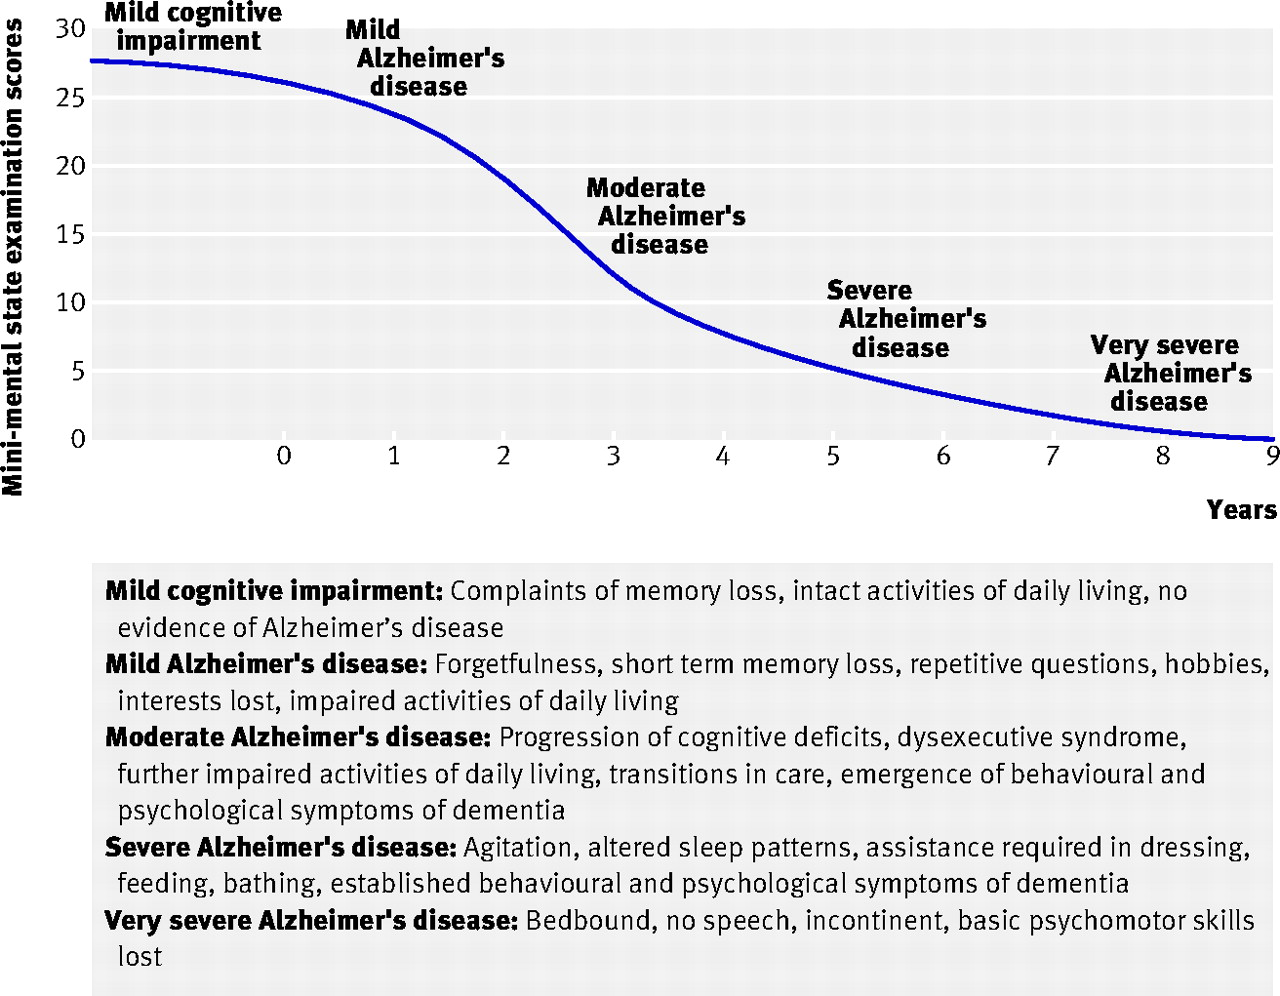
\includegraphics[width=\textwidth]{MMSEgraph.jpg}
    \caption{The progression of Alzheimer's Disease and the associated MMSE scores.\cite{Burns2009}}
    \label{fig:MMSEgraph}
\end{figure}

Although it is true that the there has been comparatively little progress in the search for an Alzheimer's cure compared to the improvement in diagnostic techniques the early diagnosis of MCI can help prevent misdiagnosis of AD and the selection of medical trial candidates. Furthermore, in the future it may allow preventative treatment to halt the progression or onset of the disease - given the modest success of late-stage intervention and the search for a cure there has been a great increase in interest concerning preventative treatment of Alzheimer's disease.\cite{Burns2009}






\section{Magnetoencephalography}

Magnetoencephalography (MEG) is a functional neuroimaging technique that measures the brain activity directly via measurement of the magnetic fields created by electrical currents at the synapses. This is a difficult task as the magnetic fields are extremely weak ($10-10^3$ fT) and thus requires the use of expensive and complicated neuromagnetometers which achieve their high sensitivity by the use of Superconducting Quantum Interference Devices (SQUIDs). Although it is worth mentioning that the first MEG recordings took place in the late 1960's before SQUIDs were available, instead using an induction coil magnetometer consisting of 2 million turns of copper wound about a ferrite core.\cite{Hari2012}

Furthermore the weakness of the magnetic fields relative to ambient magnetic noise ($10^8$ fT) requires shielding the laboratory to reduce noise. The magnetic field due to an electric current is described by Amp\`{e}re's Law and the direction can be easily determined by the right hand rule. As the magnetic field is orthogonal to the current, MEG is sensitive to the tangential component of the synaptic currents and therefore is most sensitive to pyramidal neurons near the cortical surface as pyramidal neurons have most of their currents tangential to the cortical surface and MEG is generally not sensitive to deep brain regions (although some studies have shown this may not always be the case\cite{Internationale2007}).

Despite these problems of MEG it has several advantages over other methods:

\begin{itemize}
\item It is non-invasive and has a high temporal resolution
\item Magnetic fields unlike electric fields in Electroencephalography (EEG) are not impeded by the skull, scalp etc.
\item Unlike EEG it does not require a reference signal allowing for easier source localisation\cite{Zani2002}
\item It is a direct measurement, unlike many methods such as fMRI and fNIRS which use cerebral blood flow as a proxy for neural activity

\end{itemize}

MEG recordings are often combined with anatomical MRI to enable accurate source localisation. The data processing requires the removal of artefacts which can be divided into three kinds: System related artefacts (Superconducting Quantum Interference Device (SQUID) jumps, nosiy/saturated channels etc.), external artefacts (due to power lines, mains AC etc.), physiological artefacts (due to eye movements, cardiac/muscle activity, head movement etc.). \cite{Gross2013} The visual inspection of raw data and power spectra is highly recommended although often automated/semi-automated approaches will have to be used due to the large volumes of data recorded. The way these challenges were handled in the present work will be discussed in the Methodology chapter.



\section{Previous work}


MEG has been used to investigate a wide range of brain disorders including Alzheimer's, Schizophrenia, Major Depressive Disorder and Autism. Techniques include synchrony and coherence studies (due to its high temporal resolution), Spectral ratios (the ratios of relative powers of the different frequency bands) and non-linear techniques such as complexity analysis.\cite{Williams2010}

As a result of these studies it was discovered that many brain disorders including Alzheimer's, depression, attention-deficit hyperactivity disorder and schizophrenia result in a change in the effect of ageing on brain activity as compared to healthy controls - this was described as a `rupture' in the normal evolution of the neural activity.\cite{Escudero2013}

Previous analysis on the dataset intended for use in this study found that brain oscillatory complexity (as quantified by the Lempel-Ziv Complexity algorithm) had a quadratic relationship with age.\cite{Fernandez2012} It was also discovered that spectral properties followed a similar quadratic relationship.\cite{Gomez2013}







  \chapter{Analysis of Miniature Post Synaptic Potentials}
  \chapter{Conclusion and future works}



  % Appendix
  %\appendix

  %\chapter{Tools}




  % Bibliography
  \bibliography{refs/bibliography}{}
  \bibliographystyle{apalike}
\end{document}
